%%% background to the research work
\chapter{Introduction} % at least 5 pages, not more than 10

%%%%%%%%%%%%%%%%%%%%%%%%%%%%%%%%%%%%%%%%%%%%%%%%%%%%%%%%%%%%%%%%%%%%%%%%%%%%%%%%
\section{Computer-aided Drug Discovery and Design}
  \subsection{Computational Methods}
    In the last decades, the development of new pharmaceuticals has been significantly boosted by the field of \textit{computer-aided drug discovery and design}. Computational methods allow to automate the exploration of a huge space of molecule configurations, with the goal of predicting which compounds would elicit desired biologic responses, and which others can be disregarded. According to these predictions, the molecules with the most therapeutic potential can be prioritized in further experimental stages, saving time and resources in the process of finding new benefitial drugs \cite{drug_discovery_2014}.

    Computational methods for drug discovery can be categorized in two main branches: \textit{ligand-based} (LBDD) and \textit{structure-based} (SBDD). Ligand-based methods focus only in the ligand and try to predict the behaviour of new molecules by taking as reference the activity of other known strucurally similar ligands. Structure based methods use information from the 3D structures of both ligand and target, and include approaches such as \textit{ligand docking}, \textit{molecular dynamics simulations} and \textit{pharmacophore modeling} \cite{drug_discovery_2014, structure_based_2019}.

  \subsection{Target Molecules and Binding Pockets}
    Although SBDD methods require the additional knowledge of the target structure (which is not trivial), they have been proven to be powerful and efficient methods in drug discovery \cite{structure_based_2019}. Consequently, the first basic step of SBDD methods is resolving the 3D structure of the therapeutically important \textbf{target molecule}, which traditionally refers to some protein of interest \cite{structure_based_2019}. However, this is not always the case, as in more recent years relevant RNA structures have also started to be considered as target molecules \cite{rna_targets_2022}.

    \begin{figure}[H]
      \centering
      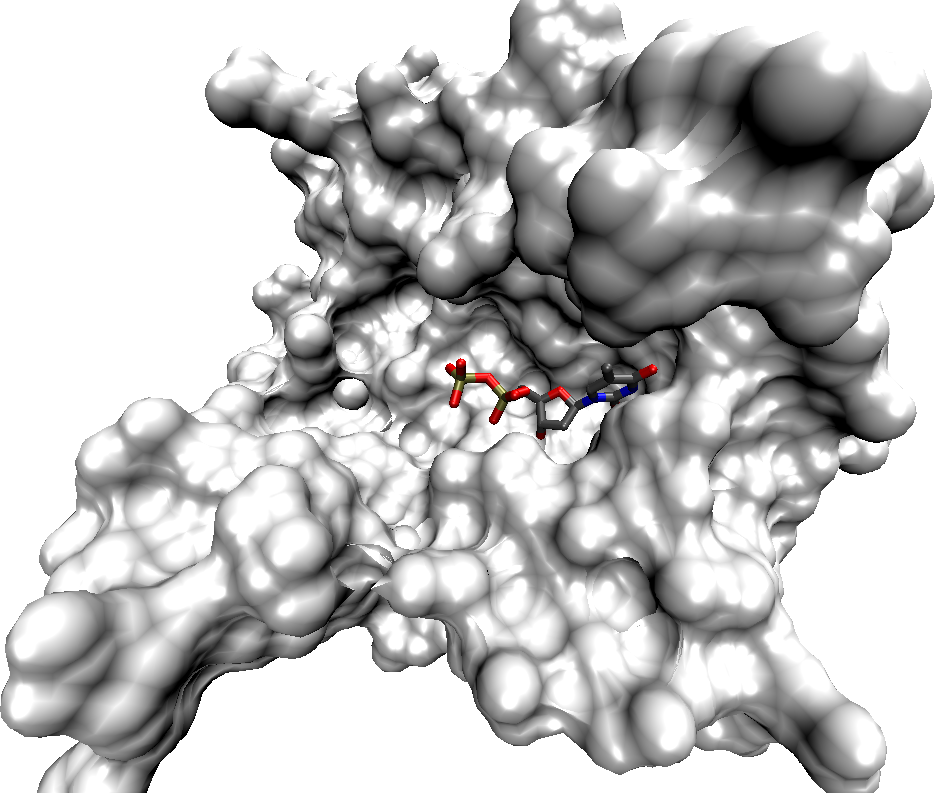
\includegraphics[width=0.5\textwidth]{figures/intro/pocket.png}
      \caption{\label{fig:intro/pocket} Ligand bound to the pocket of a protein (PDB: 1h7l).}
    \end{figure}

    Once the structure of the target is well known, an appropriate \textbf{binding pocket} must be identified. This refers to a small cavity in the target where a ligand should bind to produce the desired effect (figure \ref{fig:intro/pocket}). Once this binding site is identified, different SBDD techniques can be performed, such as \textit{virtual screening}, \textit{de novo drug design}, \textit{molecular docking} and \textit{pharmacophore modeling}, among others \cite{drug_discovery_2014, structure_based_2019, pharmacophore_and_VS_2022}.

  \subsection{Virtual Screening and Pharmacophores}
    \textbf{Virtual screening} is a series of computational methods where a dataset of chemical compounds is reduced to only those with some chemical characteristics of interest, which generally means those with higher binding affinity to a given target pocket \cite{pharmacophore_and_VS_2022, virtual_screening_2019}. Given the immense chemical space of potential ligands, with curated databases consisting of millions of compounds, blindly performing virtual screening over whole datasets is often unpractical \cite{virtual_screening_2013}. However, this process can be optimized by using \textit{pharmacophores} to reduce the search space to only those molecules that best satisfy some desired properties \cite{pharmacophore_and_VS_2022}.

    \textbf{Pharmacophore} models describe the spatial arrangement of steric and electronic features that allow ligands to optimally interact with their target binding sites \cite{pharmacophore_and_VS_2022, virtual_screening_2019, pharmacophore_modeling_2022, drug_discovery_2014}. The core idea behind pharmacophores is that ligands with common physicochemical properties and spatial arrangements should have a similar biological activity on the same target. The most relevant pharmacophoric features include \textit{positively and negatively charged groups}, \textit{aromatic groups}, \textit{hydrogen bond acceptors/donors}, \textit{hydrophobic areas}, \textit{exclusion volumes}, among others (figure \ref{fig:intro/pharmacophores}) \cite{pharmacophore_and_VS_2022, drug_discovery_2014}.

    \begin{figure}[H]
      \centering
      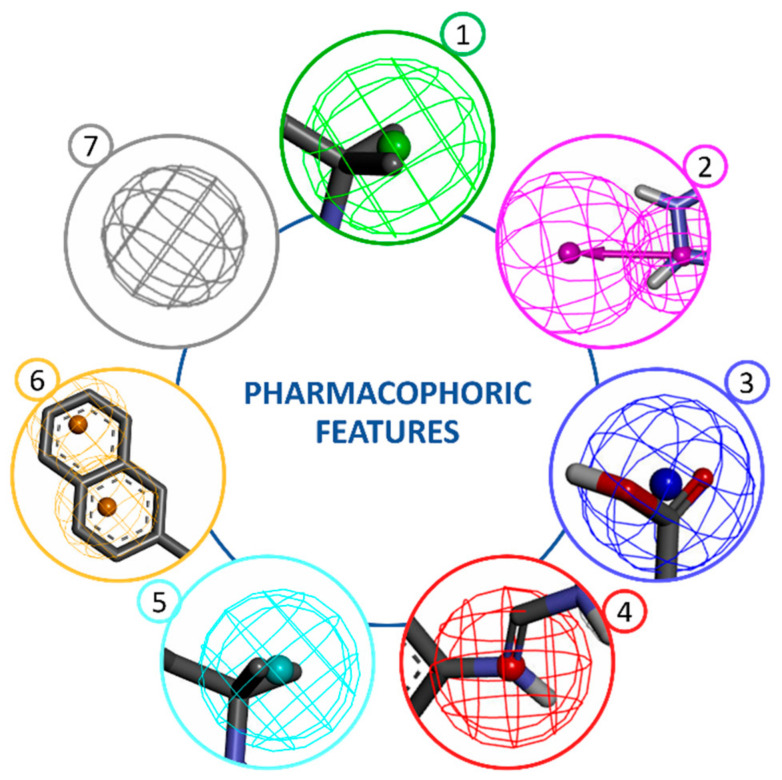
\includegraphics[width=0.5\textwidth]{figures/intro/pharmacophores.jpg}
      \caption{\label{fig:intro/pharmacophores} Summary of the main pharmacophoric features. 1) hydrogen bond acceptors, 2) hydrogen bond donors, 3) negatively charged, 4) positively charged, 5) hydrophobic, 6) aromatic, 7) exclusion volume. Adapted from \cite{pharmacophore_and_VS_2022}.}
    \end{figure}

    Pharmacophores can be modeled in either LBDD or SBDD pipelines. In the case of a structure-based approach, the pharmacophore can be obtained by different strategies. A completely target-based method can be employed, in which the pharmacophoric features are inferred by performing an analysis of the binding pocket's structure \cite{pharmacophore_and_VS_2022, virtual_screening_2019}.

    A more experimental approach involves molecular docking of different molecules from a ligand dataset, clustering the fragments with best affinity and extracting pharmacophore features from these clusters. Another straightforward and still effective strategy can be followed when experimental structures of target-ligand complexes are available. In this case, the pharmacophore features can be built based on this ligand, whose bioactive conformation is already known \cite{virtual_screening_2019}.


%%%%%%%%%%%%%%%%%%%%%%%%%%%%%%%%%%%%%%%%%%%%%%%%%%%%%%%%%%%%%%%%%%%%%%%%%%%%%%%%
\section{Physicochemical Properties of the Binding Sites}
  \subsection{Binding Affinity}
    From a chemical point of view, the interaction between ligand and target binding site can be considered as a \textit{binding reaction}, where the substrates are the ligand and the target, and the product is the target-ligand complex. The free energy of such reaction is therefore associated with how strongly the ligand binds to the target \cite{binding_affinity_2016, binding_affinity_web}.

    This concept, denominated \textbf{binding affinity}, is usually measured by the equilibrium dissociation constant $K_D$. At smaller $K_D$ values there is a greater binding affinity between ligand and target, while at larger $K_D$ values their interaction is weaker. As so, knowing which factors affect the binding affinity is key to designing optimal pocket-ligand interactions \cite{binding_affinity_web}.

    Binding affinity is mainly influenced by non-covalent intermolecular interactions between the target pocket and the ligand. This include \textit{ionic or electrostatic interactions}, \textit{stacking}, \textit{hydrogen bonds}, \textit{hydrophobic effects and van der Waals forces}, \textit{metal bonding}, \textit{desolvation}, among others \cite{binding_affinity_2016, binding_affinity_web, electrostatics_2020, stacking_binding_2020, stacking_trp_2022, hbonds_2023, hydrophobic_2017, hydrophobic_2022}.

    Computational methods behind binding affinity calculations often involve \textbf{energy functions}, which are based either on a physical description of these interactions or on statistical analyses of experimentally characterized ligands. \textit{Physical energy functions} can contain terms common in molecular dynamics force fields, such as: bond stretching; angles bending, rotation and torsion; coulombic interactions; van der Waals attraction; exchange repulsion and others. On the other hand, \textit{statistical energy functions} often rely on distances between atoms to build an empirical potential of mean force, by taking into account the physicochemical properties that affect binding affinity \cite{binding_affinity_2016}.

  \subsection{Electrostatics}
    Binding affinity is greatly affected by the \textbf{electrostatic interactions} between positively and negatively charged groups in oposing molecules (figure \ref{fig:intro/electrostatics}). This contribution is even higher when intermolecular ion pairs (salt bridges) are formed. It is important to note that under physiological conditions, the presence of ions in the solvent further impact the electrostatic behaviour of the molecules. As RNA molecules are highly negatively charged, cations tend to condense near their surface. On the other hand, proteins tend to attract both anions and cations, but with less intensity. Either way, the long range nature of electrostatic forces and the abundance of charged amino and nucleic acids make these interactions particularly relevant \cite{electrostatics_2020, electrostatics_2019, apbs_2004}.

    \begin{figure}[H]
      \centering
      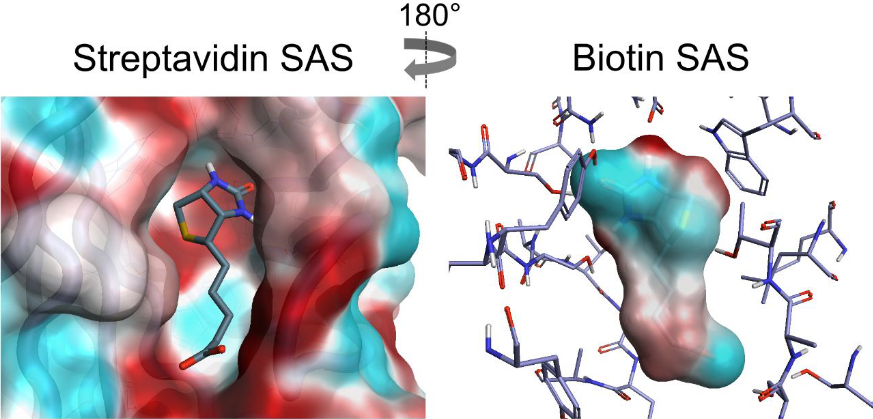
\includegraphics[width=0.5\textwidth]{figures/intro/electrostatics.png}
      \caption{\label{fig:intro/electrostatics} Electrostatic interaction between ligand (biotin) and target protein (streptavidin) forming a complex (PDB: 3RY2). Blue) negative electrostatic potential, Red) positive electrostatic potential. Adapted from \cite{electrostatics_2019}.}
    \end{figure}

    A standard method for studying biomolecular electrostatics consists of solving the Poisson-Boltzmann equation of continuum electrostatics, which incorporates information about the molecular shape and charge distribution. This is best solved numerically with a grid-based and finitely-discretized approach. The \textbf{Adaptive Poisson–Boltzmann Solver} (APBS) software provides a flexible and powerful pipeline for this purpose \cite{apbs_2004, apbs_2018, apbs_web, umol_apbs_2020}.

  \subsection{Stacking}
    The presence of $\pi$-stacking interactions can also contribute to a higher affinity in ligand binding. This kind of interaction is traditionally considered to happen between two \textit{aromatic groups}, which are notable for their planarity and $\pi$-electron cloud over and under the aromatic ring plane. Whenever the spatial placement allow for these clouds to interact in a particular way, a \textbf{stacking interaction} occurs. The chemical details behind this phenomenon are still not fully understood and are still object of debate, which also means their quantification and modeling is not straightforward \cite{stacking_binding_2020, stacking_trp_2022, stacking_general_2020}.

    \begin{figure}[H]
      \centering
      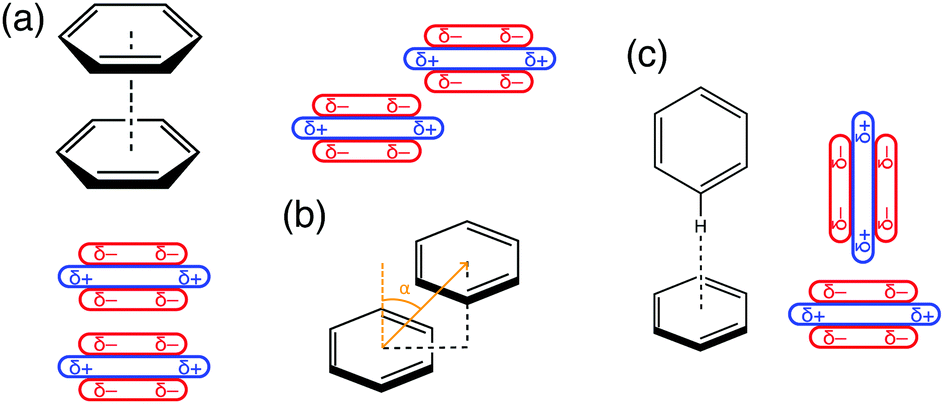
\includegraphics[width=0.5\textwidth]{figures/intro/stacking_configs.png}
      \caption{\label{fig:intro/stacking_configs} Common theoretical configurations for stacking interactions. a) "sandwich" interaction, b) parallel-offset, c) perpendicular. Adapted from \cite{stacking_general_2020}.}
    \end{figure}

    The spatial configuration of the aromatic rings plays a fundamental role in stacking interactions. This can be summarized by three spatial degrees of freedom: distance, $\alpha$ angle and $\beta$ angle. The $\alpha$ angle describes how tilted the center of geometry is from one ring with respect to the other ring, while $\beta$ is the angle between the vectors normal to the planes (figures \ref{fig:intro/stacking_configs} and \ref{fig:intro/stacking_angles}) \cite{stacking_general_2020, rna_2015, aromatic_2018}.

    \begin{figure}[H]
      \centering
      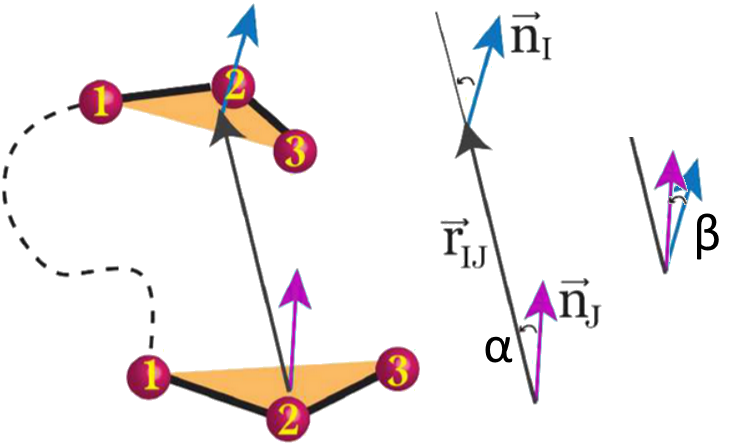
\includegraphics[width=0.5\textwidth]{figures/intro/stacking_angles.png}
      \caption{\label{fig:intro/stacking_angles} $\alpha$ and $\beta$ angles between the aromatic planes in stacking interactions. Adapted from \cite{rna_2015}.}
    \end{figure}

    The traditional \textbf{$\pi$-$\pi$ stacking} is considered to be optimal when $0^{\circ} < \alpha << 90^{\circ}$ and $\beta \approx 0^{\circ}$, yielding a \textit{parallel-offset} geometry. The alternative \textbf{CH-$\pi$ stacking} also represents an energetic local minimum, with $\alpha \approx 0^{\circ}$ and $\beta \approx 90^{\circ}$, which corresponds to a \textit{perpendicular} geometry (figure \ref{fig:intro/stacking_configs}) \cite{stacking_general_2020}. It is also noteworthy that aromatic rings can also interact in other similar ways to $\pi$-$\pi$ and CH-$\pi$ stacking. These include \textit{cation-$\pi$}, \textit{amid-$\pi$}, \textit{amid-$\pi$} and \textit{halogen-$\pi$} \cite{stacking_binding_2020, electrostatics_2020}.

  \subsection{Hydrogen Bonds}
    Another kind of interaction fundamental for the structure of macromolecules and their binding affinity to ligands is the presence of \textbf{hydrogen bonds}. These are weak interactions that happen between so-called \textit{donor} and \textit{acceptor} atom pairs, under an appropriate distance and angle. A \textbf{donor} is an electronegative atom such as nitrogen (N), oxygen (O) or fluor (F) covalently bound to a hydrogen (H) atom, while an \textbf{acceptor} is an electronegative atom with a lone pair of electrons or a negative charge (figure \ref{fig:intro/hbonds}) \cite{hbonds_2023}.

    \begin{figure}[H]
      \centering
      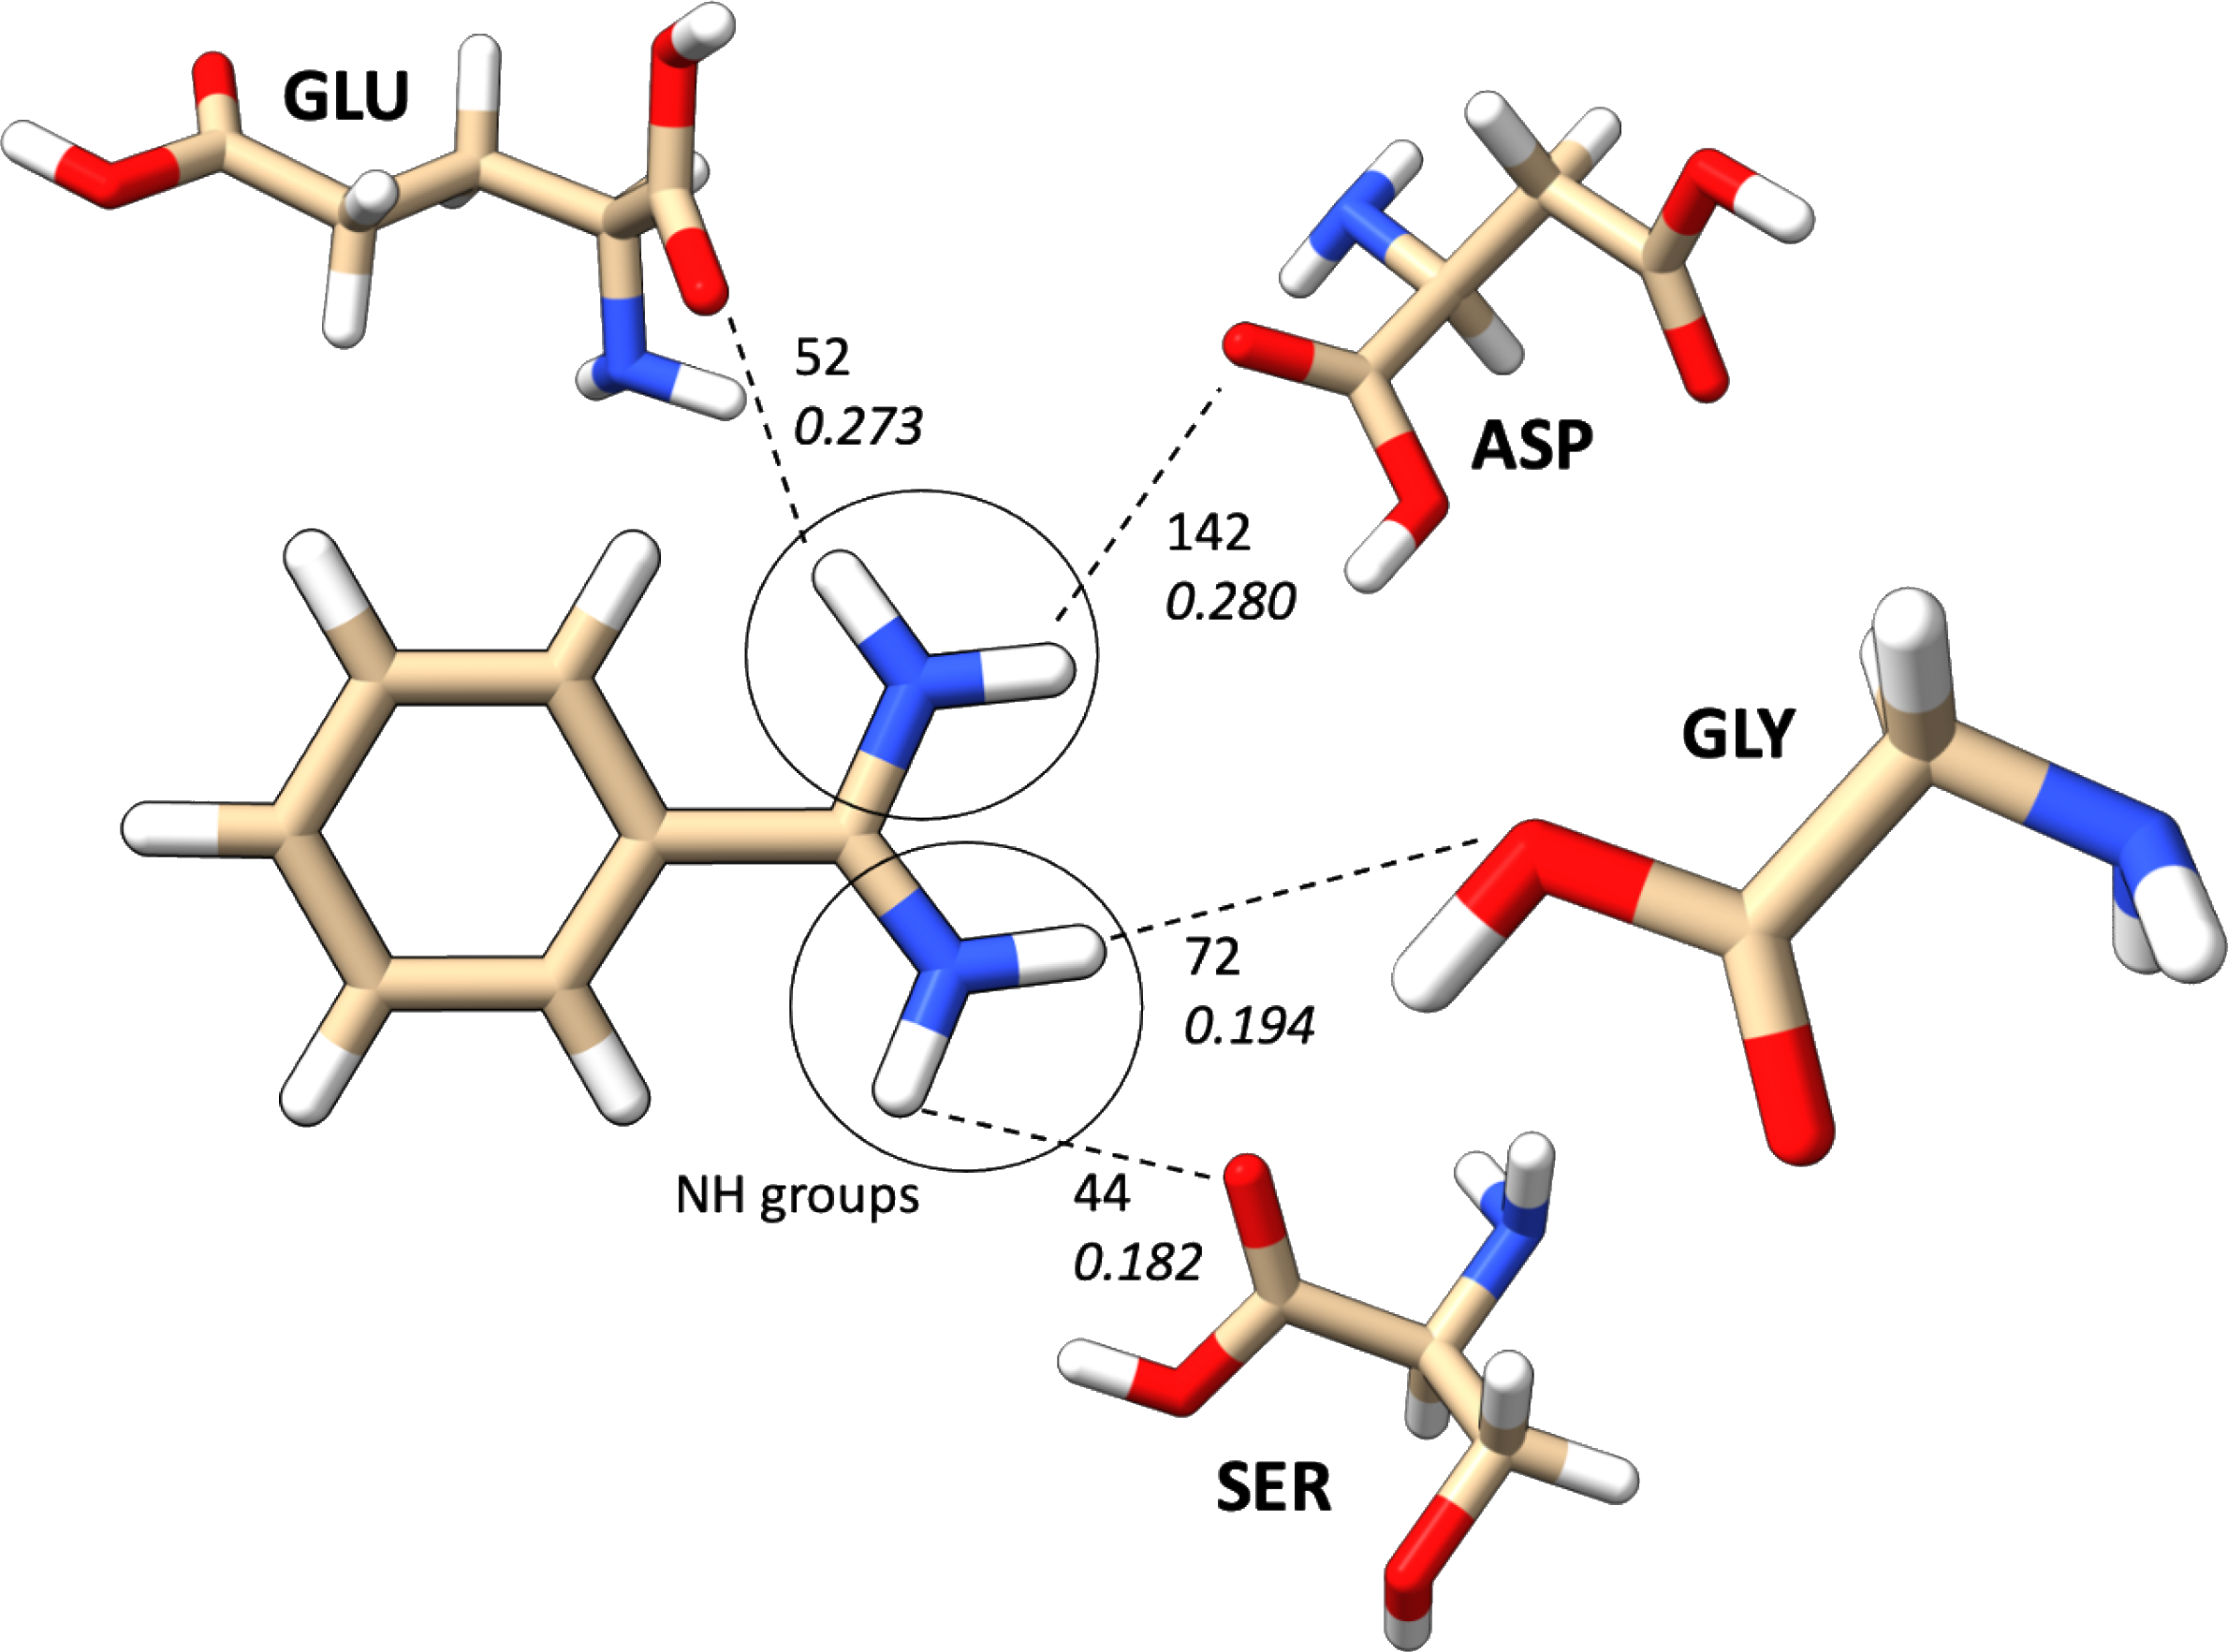
\includegraphics[width=0.5\textwidth]{figures/intro/hbonds.png}
      \caption{\label{fig:intro/hbonds} Hydrogen bond interactions between N-H groups acting as donors and oxygen atoms from aminoacids acting as receptors. Adapted from \cite{hbonds_2023}.}
    \end{figure}

    In proteins, oxygen and nitrogen atoms in both the backbone of the polypeptide and in the functional group of the aminoacids can act as donors or acceptors. The most common hydrogen bond interactions in proteins are of the form N-H...O, while O-H...O and N-H...N can also be commonly observed \cite{hbonds_2023}. In RNA, oxygen and nitrogen atoms in the nucleic bases take these roles (which oftentimes leads to the notorious \textit{base pair} interactions) \cite{rna_2015}, while oxygen atoms in the phosphate groups of their backbone could also act as acceptors in some cases \cite{hbonds_2023} (figure \ref{fig:intro/hbonds_po}).

    \begin{figure}[H]
      \centering
      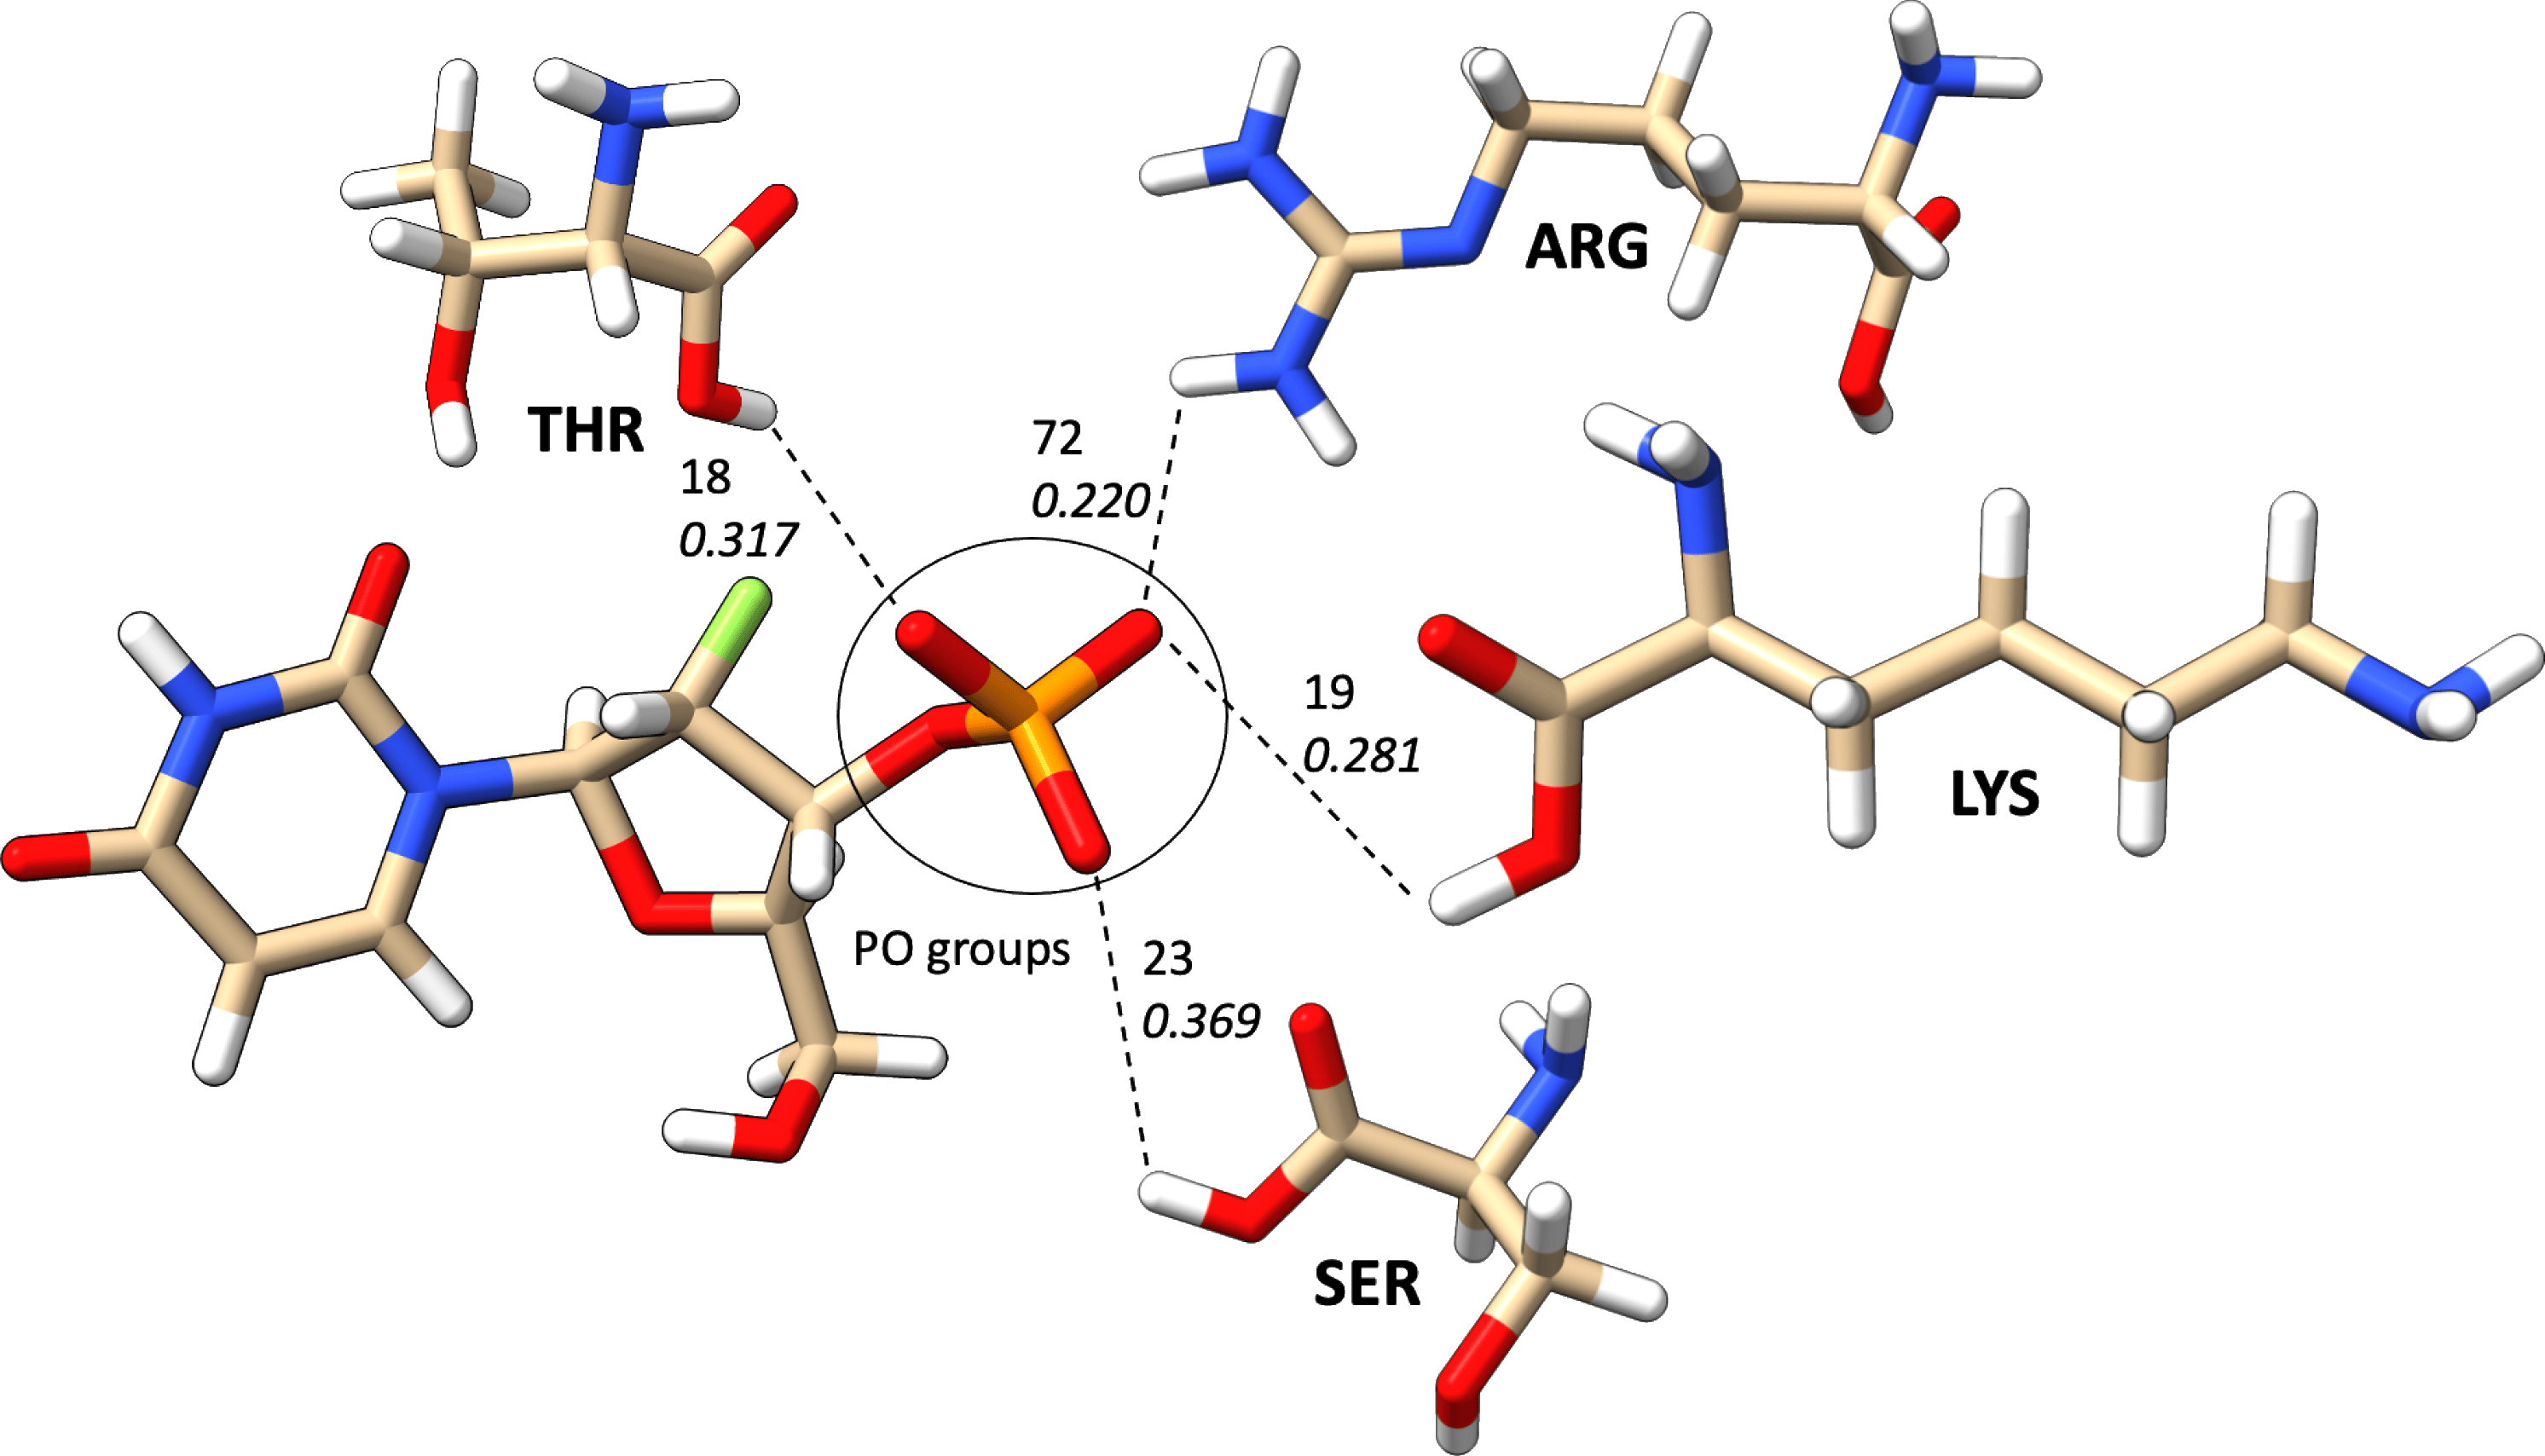
\includegraphics[width=0.5\textwidth]{figures/intro/hbonds_po.png}
      \caption{\label{fig:intro/hbonds_po} Hydrogen bond interactions between N-H and O-H groups acting as donors and a phosphate group acting as receptor. Adapted from \cite{hbonds_2023}.}
    \end{figure}

  \subsection{Hydrophobicity}
    The arrangement or displacement of water molecules near the surfaces of targets and ligands is also a very relevant factor that affects binding affinity \cite{hydrophobic_2017, hydrophobic_2022}. In structural terms, the dynamics of water can affect the structure and rigidity of the macromolecules, which sometimes affects the shape and flexibility of the pockets and therefore their binding affinity \cite{hydrophobic_2022}. In some instances, water is displaced from specific regions and energetically favorable interactions between non-polar groups emerge, which is commonly known as the \textbf{hydrophobic effect}. Hydrophobicity is mostly relevant in the case of some target proteins, where it is commonly associated to the formation of these \textit{solvent exclusion} (water displacement) cavities, usually buried inside the protein to avoid contact with the outside water (figure \ref{fig:intro/hydrophobic}) \cite{hydrophobic_2017}.

    \begin{figure}[H]
      \centering
      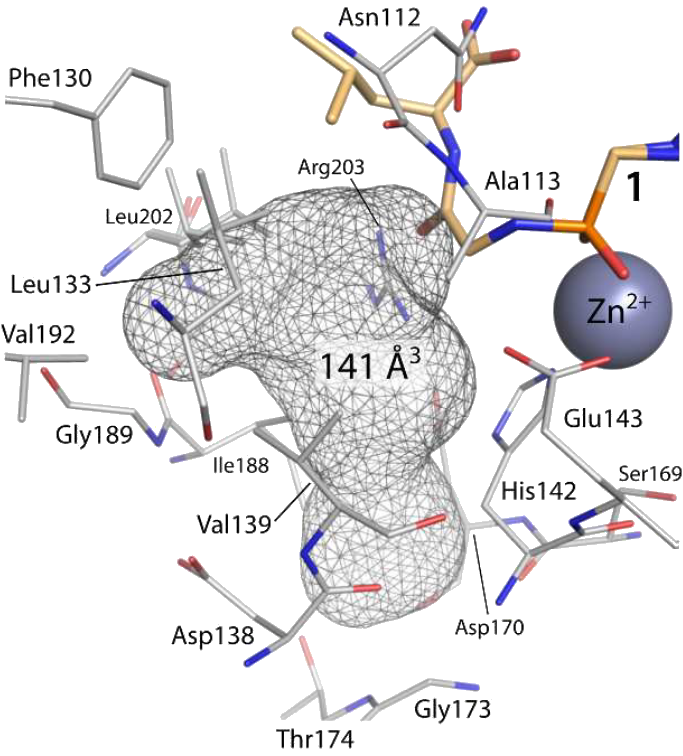
\includegraphics[width=0.5\textwidth]{figures/intro/hydrophobic.png}
      \caption{\label{fig:intro/hydrophobic} Volumetric representation of a solvent exclusion cavity inside of a metalloprotease (thermolysin). Adapted from \cite{hydrophobic_2017}.}
    \end{figure}


%%%%%%%%%%%%%%%%%%%%%%%%%%%%%%%%%%%%%%%%%%%%%%%%%%%%%%%%%%%%%%%%%%%%%%%%%%%%%%%%
\section{Molecular Visualization}
  \subsection{Molecular Visualization Software}
    Due to the nanoscopic nature of molecules, the field of molecular biology relies heavily on computational technologies to collect and gather insights from the structures and behaviour of these tiny systems. A great source of qualitative analysis and insight out of these data is enabled by the great variety of \textbf{molecular visualization software} and techniques that have been developed over the decades \cite{visualization_2018}.

    Molecular visualization is a huge topic constantly in evolution, with different parties developing different software packages or techniques to approach general or specific visualization purposes. Some of the most consolidated software environments are \textit{Chimera}, \textit{PyMOL}, \textit{PMV} and \textit{VMD} \cite{visualization_2018, vmd_96}. The Protein Data Bank lists a great variety of other software related to molecular graphics: \textit{BioBlender}, \textit{BioViz Studio}, \textit{CCP4mg}, \textit{Cn3D}, \textit{CrystalMaker}, \textit{ePMV}, \textit{EzMol}, \textit{Foldit}, \textit{ICM-Browser}, \textit{IcmJS}, \textit{iMol}, \textit{Jmol}, \textit{Mage and Kinemages}, \textit{Marvin}, \textit{MembraneEditor}, \textit{MOE}, \textit{Molecule World}, \textit{Molecules}, \textit{MolScript}, \textit{MolviZ.org}, \textit{Nanome}, \textit{PDBWORDS}, \textit{Perse Visualizer}, \textit{POLYVIEW}, \textit{Prosat}, \textit{Protein Imager}, \textit{QTree}, \textit{QuteMol}, \textit{RasMol}, \textit{Raster3D}, \textit{RasTop}, \textit{RCSB MBT Viewers}, \textit{RmscopII}, \textit{Schrödinger Product Suites}, \textit{SPADE}, \textit{STRAP}, \textit{Swiss PDB viewer}, \textit{UGENE}, \textit{WebMol}, \textit{YASARA}, \textit{Zeus} and \textit{ZMM} \cite{visualization_web}.

    Molecular visualization involves dealing with complex three-dimensional graphical data, oftentimes in a high-performant interactive way, which for large systems can be very computationally expensive. This challenge is shared with other fields in multimedia development, a notable one being the videogame industry. To take advantage of the highly optimized techniques used in videogame development, some molecular visualization tools have been built on top of \textit{game engines}. Tools such as \textit{UnityMol} \cite{unitymol_2015, unitymol_web}, \textit{UDock} and \textit{CellVIEW} have been built using the notorious game engine \textit{Unity3D} \cite{visualization_2018, unity_2014}.

    \begin{figure}[H]
      \centering
      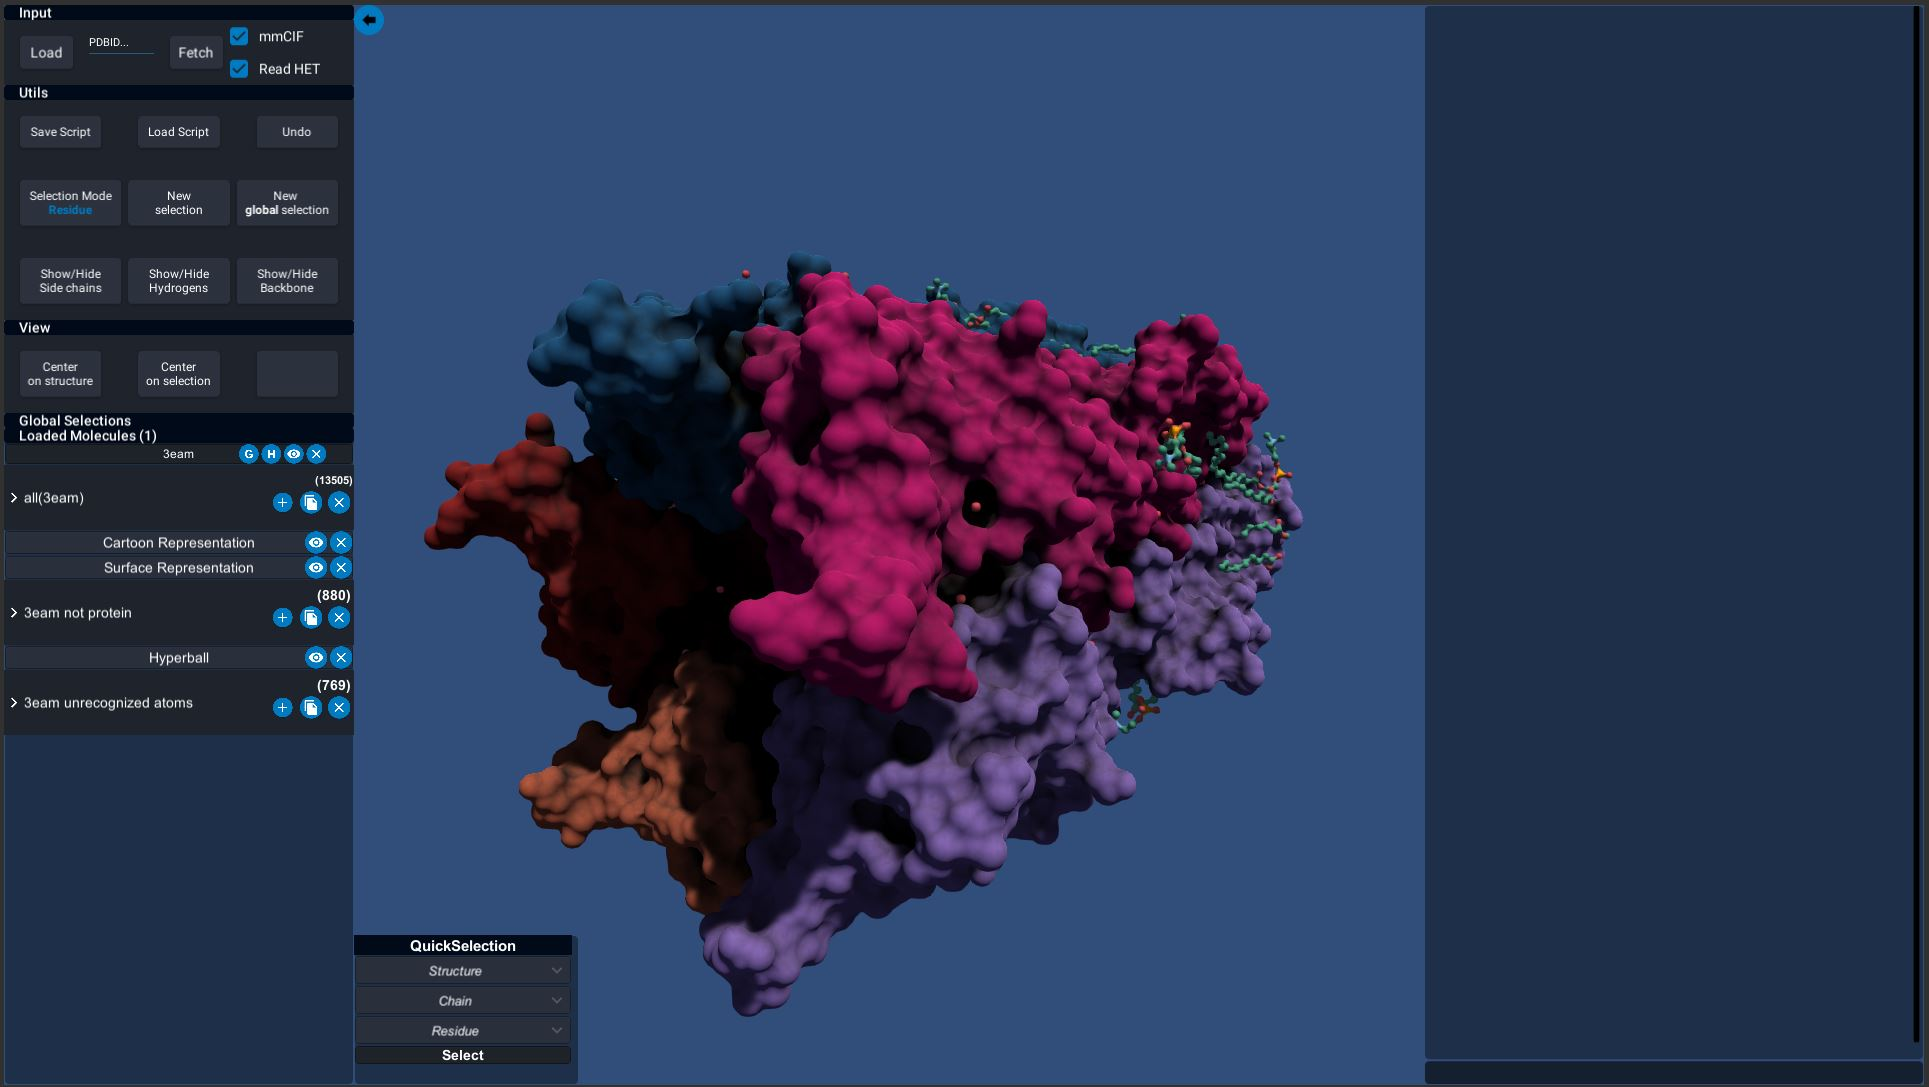
\includegraphics[width=0.5\textwidth]{figures/intro/unitymol.jpg}
      \caption{\label{fig:intro/unitymol} Visualization of a protein interacting with ligands using UnityMol. Adapted from \cite{unitymol_web}.}
    \end{figure}

    The molecular viewer \textbf{UnityMol} covers the basic functionalities of molecular visualization (figure \ref{fig:intro/unitymol}), while also serving as an environment for prototyping new representation techniques for specific systems or properties. It can be used to visualize proteins, nucleic acids, polysaccharides, ligands, molecular dynamics trajectories, among others. It also takes advantage of graphical and computational resources provided by the engine, such as shader GPU programs (for optimized structure representations) and the VRTK framework (for developing a \textit{virtual reality} approach to molecular visualization) \cite{unitymol_2015, unitymol_web}.

  \subsection{Molecular Representations}
    Molecular visualizers employ different data visualization techniques to portray the structural and physicochemical information of the biological systems in an intuitive and ergonomic way. Visual cues are exploited for this purpose, such as shapes, contours, color-codes, opacities, labels, animations (in the case of molecular dynamics trajectories), among others. These tecnhiques allow to build \textbf{representations} of the molecules, called this way because they seek to represent the spatial three-dimensional data into an intuitive and tangent object that can be observed and interacted with. Classical examples of representations include \textit{ball and stick}, \textit{cartoon}, \textit{licorice}, \textit{line}, \textit{point}, \textit{ribbon}, \textit{rocket}, \textit{spacefill}, \textit{surface} and \textit{trace} (note that names can change on different software implementations) \cite{representations_web}. Insightful observations can be obtained by alternating between these representations in different parts of a molecular system of interest.

    \begin{figure}[H]
      \centering
      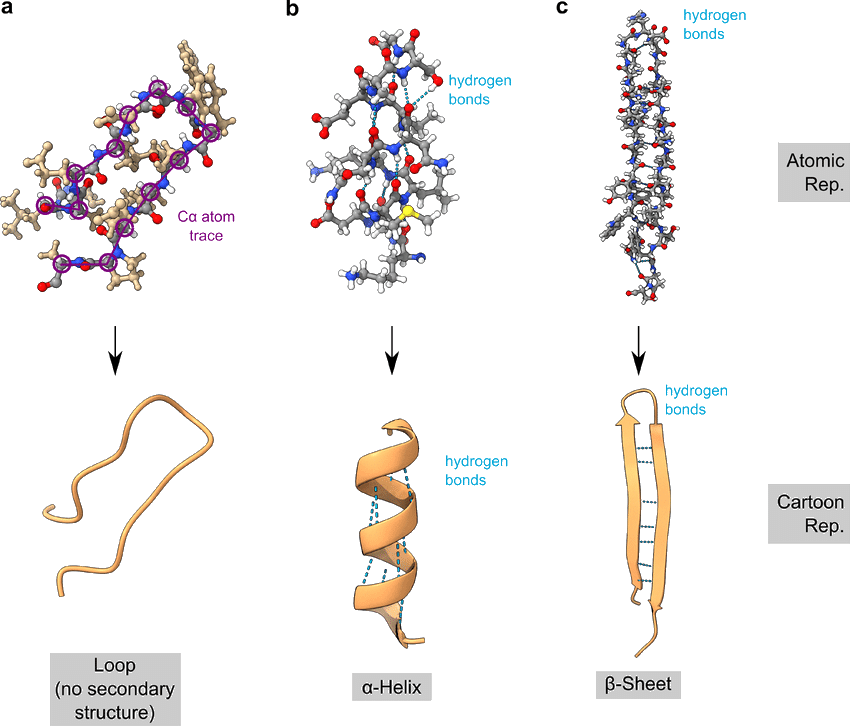
\includegraphics[width=0.5\textwidth]{figures/intro/rep_cartoon.png}
      \caption{\label{fig:intro/rep_cartoon} Example of a mix between the \textit{licorice} and \textit{ball and stick} representations (top) and the \textit{cartoon} representation (bottom) of polypeptides. Adapted from \cite{representations_2021}.}
    \end{figure}

    The \textbf{licorice} representation highlights the \textit{bond topology} of the molecules and is often color coded according to each atom, so it is best suited for small molecule ligands or closeups of pocket structures (figures \ref{fig:intro/pocket}, \ref{fig:intro/pharmacophores}, \ref{fig:intro/electrostatics}, \ref{fig:intro/hbonds}, \ref{fig:intro/hbonds_po}, \ref{fig:intro/hydrophobic}, \ref{fig:intro/unitymol}, \ref{fig:intro/rep_cartoon}, \ref{fig:intro/rep_surfaces}). The \textbf{cartoon} representation summarizes the \textit{secondary structure} of macromolecules into simpler shapes. This is usually associated to proteins (figures \ref{fig:intro/rep_cartoon}, \ref{fig:intro/rep_surfaces}) but can also be applied to nucleic acids, polysaccharides, lipids and other macromolecules.

    For the \textbf{surface} representations, the volume occupied by the electronic clouds of the atoms is estimated by an algorithm, then a contour is drawn around this volume to obtain a tangible shape that emphasizes the overall \textit{three-dimensional shape} of the molecule (figures \ref{fig:intro/pocket}, \ref{fig:intro/electrostatics}, \ref{fig:intro/unitymol}, \ref{fig:intro/rep_surfaces}). More or less precise algorithms can be used to calculate this estimation, depending if precision or performance is to be prioritized. Alternatively, a \textbf{spacefill} representation can be employed, where a sphere is drawn around each atom with a theoretical radius that depends on the element (figures \ref{fig:intro/hydrophobic}, \ref{fig:intro/rep_surfaces}).

  \subsection{Visualization of Physicochemical Properties}
    Apart from the spatial configuration of the molecules, the physicochemical properties of the system are also of interest for many applications, such as protein-ligand interactions. As such, the visualization of these data should also be considered when developing molecular visualizers. The \textbf{electrostatics} of the molecules is usually portrayed by color-coding surface representations, where different colors correspond to different sign and intensity of surface charges (figures \ref{fig:intro/electrostatics}, \ref{fig:intro/rep_surfaces}.c). Similarly, \textbf{hydrophobicity} is many times also represented by color-coding the surfaces of the molecules, according to theoretical or empirical hydrophobic qualities of the residues or functional groups involved (figure \ref{fig:intro/rep_surfaces}.b).

    \begin{figure}[H]
      \centering
      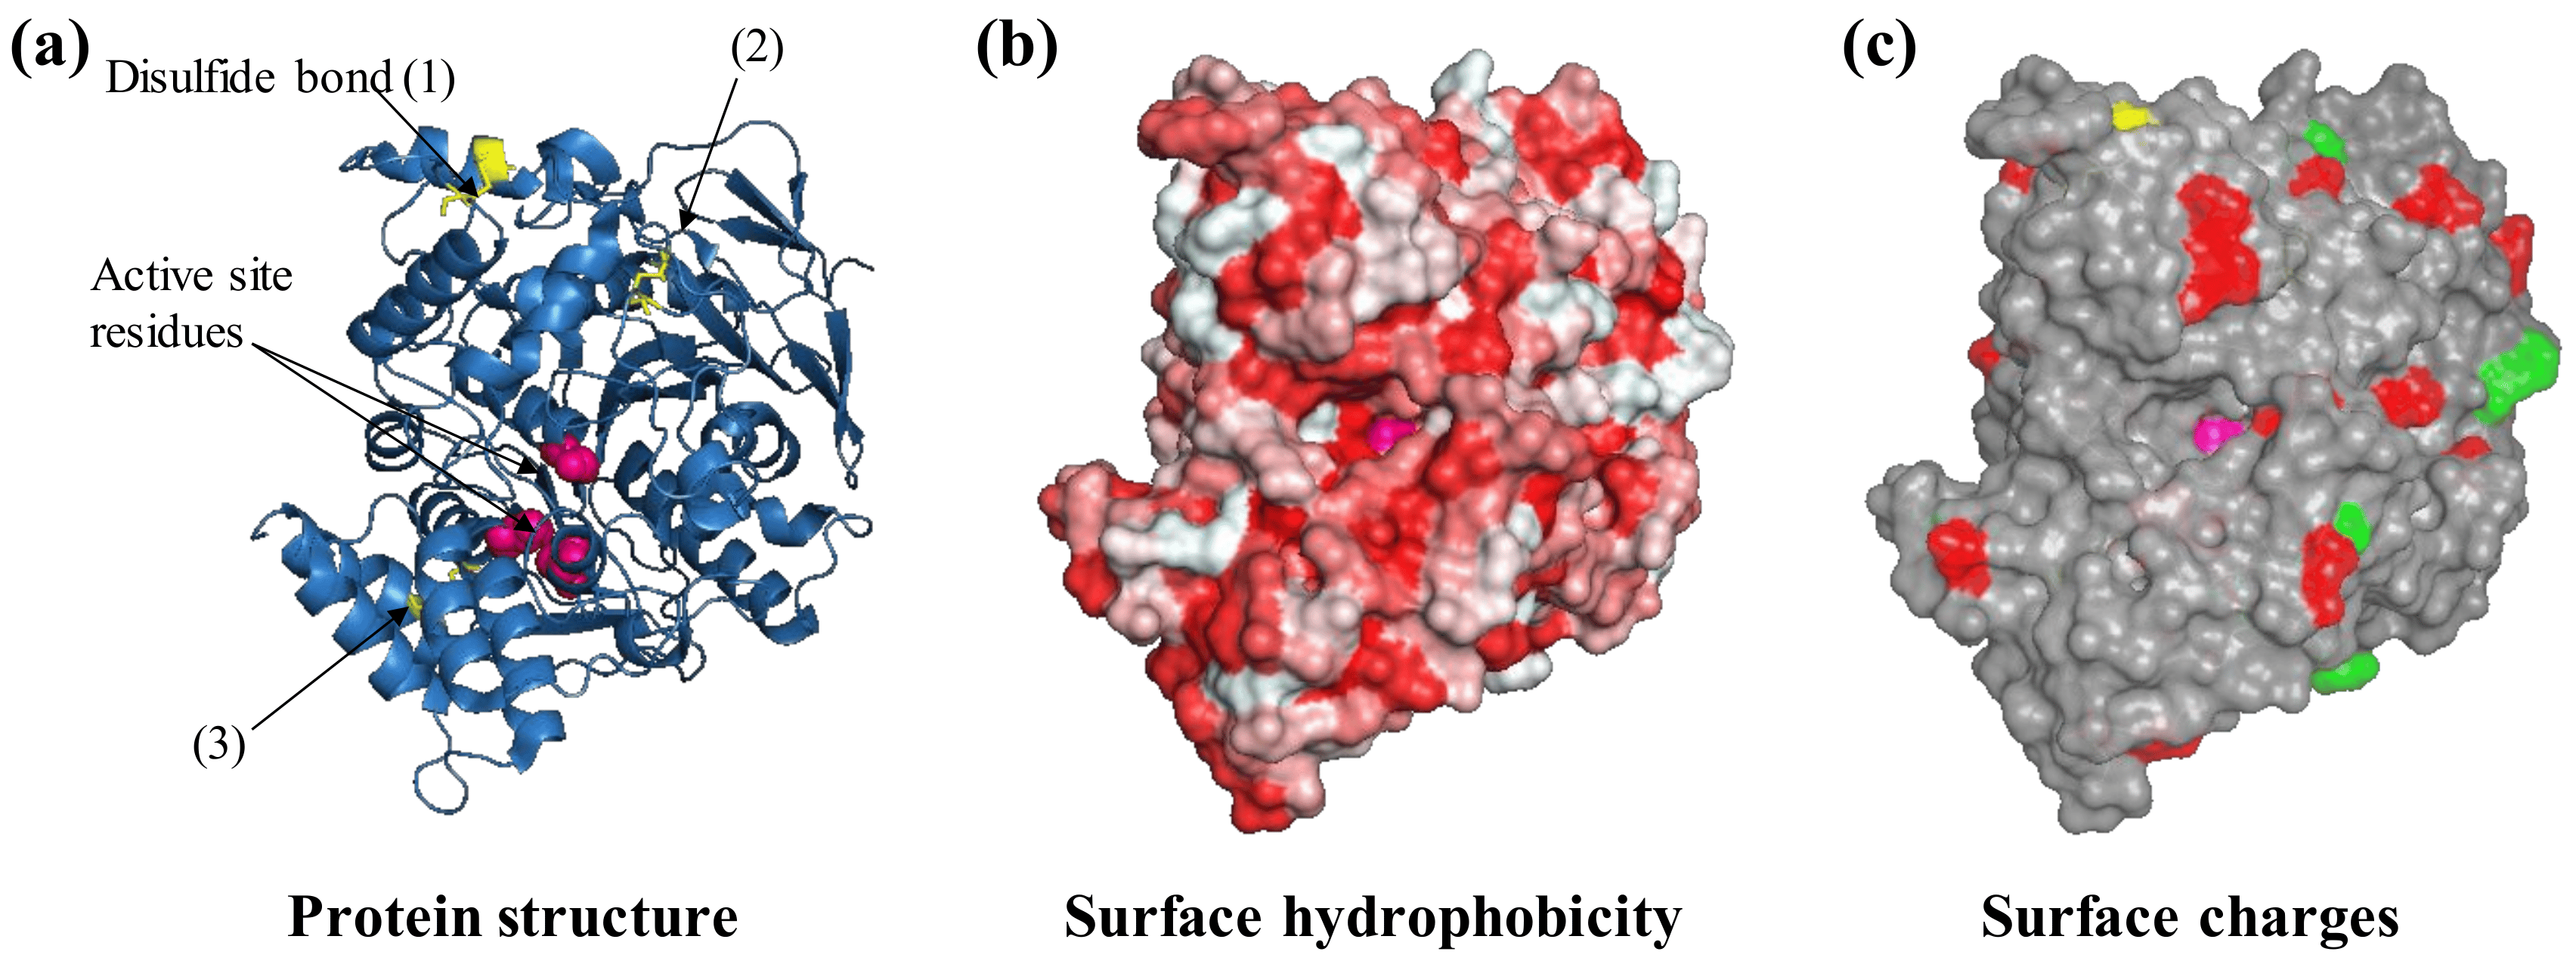
\includegraphics[width=0.8\textwidth]{figures/intro/rep_surfaces.png}
      \caption{\label{fig:intro/rep_surfaces} Example of different representations of a protein. a) cartoon representation, b) surface representation with hydrophobicity as color code, c) surface representation with electrostatics as color code. Adapted from \cite{representations_2018}.}
    \end{figure}

    In the case of \textbf{hydrogen bonds}, the common approach is to represent them as dotted lines between the acceptor and donor atoms (figures \ref{fig:intro/hbonds}, \ref{fig:intro/hbonds_po}, \ref{fig:intro/rep_cartoon}). On the other hand, \textbf{stacking} interactions are not usually represented in any particular way. Instead, visualizers rely on the users to observe the proximity and positioning between aromatic rings and judge in an approximate manner whether stacking can be present or not.

    Interestingly, visualizers tend to focus on \textit{surface} representations when displaying physicochemical properties. However, some of these properties are inherently \textit{volumetric}, such as electrostatics and hydrophobicity. Also, when studying pocket-ligand interactions, pharmacophores further encapsulate hydrogen bonds and stacking as elements that occupy a volume of propensity. Indeed, the volume surrounded by the target pocket can be considered to contain the physicochemical properties required to study and design target-ligand interactions, but this is not exploited much in current molecular visualization.

    \begin{figure}[H]
      \centering
      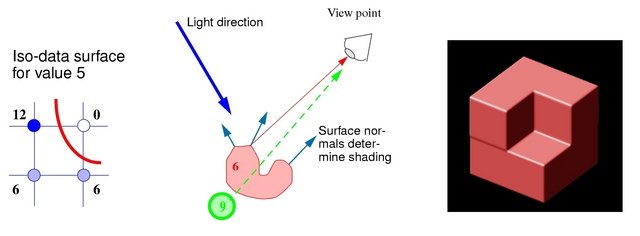
\includegraphics[width=0.8\textwidth]{figures/intro/isosurfaces.png}
      \caption{\label{fig:intro/isosurfaces} General concept of an isosurface representation to visualize two or three dimensional data. Adapted from \cite{isosurfaces_web}.}
    \end{figure}

    A notable exception is the use of a volumetric representation known as \textbf{isosurface}. This technique for visualizing three-dimensional grids of data use an adjustable treshold value to draw a contour around points with similar values, which yields a representation similar to a \textit{surface} one (figure \ref{fig:intro/isosurfaces}) \cite{isosurfaces_web}. Isosurfaces are sometimes used to represent solvent exclusion cavities when studying the hydrophobicity of a system (figure \ref{fig:intro/hydrophobic}).

    \begin{figure}[H]
      \centering
      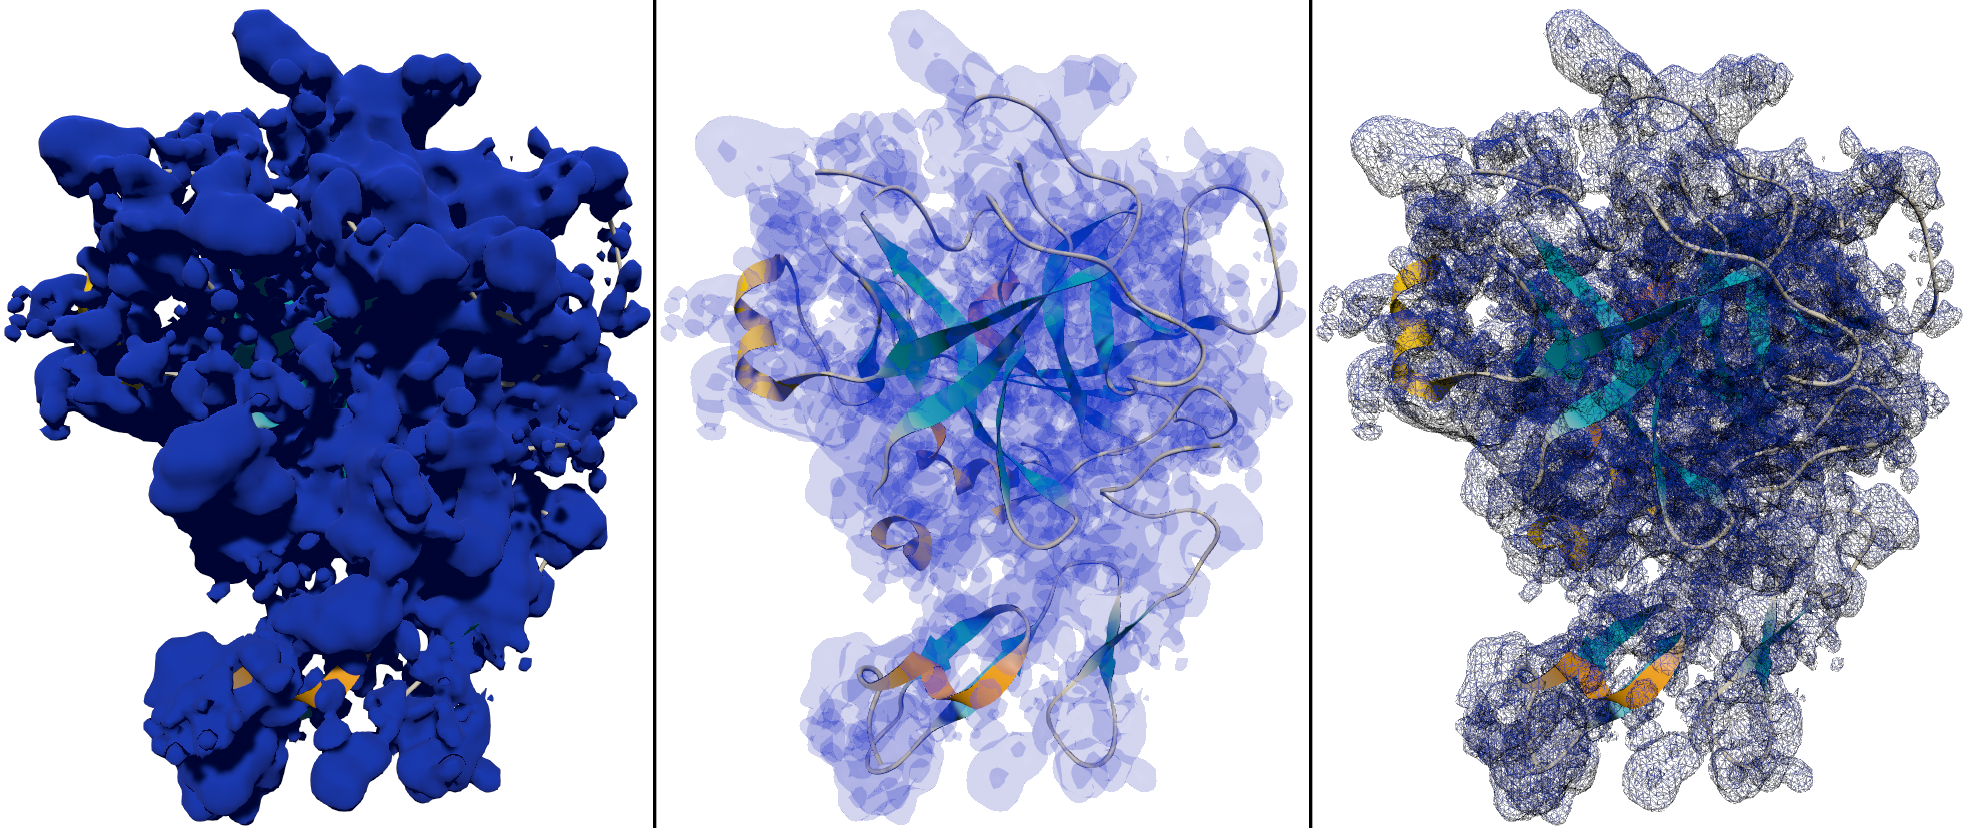
\includegraphics[width=0.8\textwidth]{figures/intro/isosurfaces_umol.png}
      \caption{\label{fig:intro/isosurfaces_umol} Isosurface representations of the whole APBS grid for a protein system. The isosurface cutoff value was set to $5$, so positive charges are being displayed. Left) solid, Middle) translucid, Right) wireframe. PDB: 1IQJ. Rendered in UnityMol.}
    \end{figure}

    There is already an implementation for isosurfaces in UnityMol, originally implemented for visualization of APBS potential grids for the whole system \cite{umol_apbs_2020}. As any other representation, UnityMol allows to configure the display of the isosurfaces in different ways. Notably, there is the possibility to draw them using \textit{solid}, \textit{translucid} or \textit{wireframe} renderings, among others, as portrayed in figure \ref{fig:intro/isosurfaces_umol}.



%%%%%%%%%%%%%%%%%%%%%%%%%%%%%%%%%%%%%%%%%%%%%%%%%%%%%%%%%%%%%%%%%%%%%%%%%%%%%%%%
